% Fra forsiden: CLRS refererer til kursets lærebog, Introduction to Algorithms, 3. udgave.
\section*{Multiple-choice}\label{sec:mc}

Dine svar skal indtastes i ITX-systemets multiple-choice modul.

\multiplechoicestart


\spoergsmaal{MergeSort og sammenligninger}
Betragt følgende input til {\sc MergeSort}, implementeret som i CLRS sektion 2.3.
\begin{center}
\begin{tabular}{|c|c|c|c|c|c|c|c|}
\hline
42 & 33 & 36 & 43 & 11 & 38 & 22 & 66\\
\hline
\end{tabular}
\end{center}
Hvor mange gange sammenligner {\sc MergeSort} elementet 42 med et andet element i input? (Sammenligninger med $\infty$ skal ikke tælles med.)
\etsvar
\mulighederstart
\svar 3 sammenligninger
\svar 4 sammenligninger
\svar 5 sammenligninger \korrekt
\svar 6 sammenligninger
\svar 7 sammenligninger
\mulighederslut
\forklaring{Vi kan fokusere på de sorterede lister hvor 42 indgår. Der laves 1 sammenligning for at lave den sorterede liste med 2 elementer, 2 sammenligninger for at lave den sorterede liste med 4 elementer, og yderligere 2 sammenligninger for at lave den endelige sorterede liste. Totalt 5 sammenligninger.}
% 42 33 36 43 11 38 22 66
% 33 42 36 43 11 38 22 66  1 sammenligning
% 33 36 42 43 11 22 38 66  2 sammenligninger
% 11 22 33 36 38 42 43 66  2 sammenligninger


\spoergsmaal{MergeSort}
Antag at {\sc MergeSort}$(A,p,r)$, implementeret som i CLRS sektion 2.3, bliver kaldt på 21 elementer (dvs. $r-p+1 = 21$).
Hvor mange kald bliver der totalt lavet til {\sc Merge-Sort}?
\etsvar
\mulighederstart
\svar 11
\svar 21
\svar 31
\svar 41 \korrekt
\svar 51
\mulighederslut
\forklaring{Antal elementer i hvert kald af mergesort, opdelt efter rekursionsniveau, er: 21; 10, 11;5, 5, 5, 6; 2, 3, 2, 3, 2, 3, 3, 3; 1, 1, 1, 2, 1, 1, 1, 2, 1, 1, 1, 2, 1, 2, 1, 2; 1, 1, 1, 1, 1, 1, 1, 1, 1, 1. Antal kald er altså $1+2+4+8+16+10 = 41$. Alternativt kan man se at det totale antal knuder i et binært træ med 21 blade, hvor alle indre knuder har to børn, altid er $2\cdot 21 - 1 = 41$.}


\spoergsmaal{Korteste-veje træ}
Betragt et korteste veje problem (eng.~\emph{single-source shortest-paths problem}) på en graf $G=(V,E)$ 
med vægtfunktion $w: E\rightarrow \mathbb{R}$ og startknude $s$. 
Hvilke af følgende egenskaber har et korteste-veje træ (eng.~\emph{shortest-paths tree}) $G'=(V',E')$ altid?
\fleresvar
\mulighederstart
\svar I $G'$ kan alle knuder i $V$ nås fra $s$.
\svar Knuden $s$ har kun udgående kanter i $G'$. \korrekt
\svar $G'$ har $|V'|-1$ kanter. \korrekt
\svar Hvis alle vægte er unikke indeholder $G'$ de $|E'|$ kanter i $G$, der har lavest vægt.
\svar $G'$ indeholder den kant i $G$, der har lavest vægt.
\mulighederslut
\forklaring{$G'$ forbinder kun $s$ med de knuder i $V$ hvortil der findes en vej i $G$.
Der er kun udgående kanter fra $s$ fordi træet ikke har nogen cykler.
$G'$ er et træ, og derfor er antal kanter lig med antal knuder minus 1.
En lav vægt er ikke en garanti for at være med i en korteste vej fra $s$ --- for eksempel kan visse kanter ikke nås fra~$s$.
}


\spoergsmaal{Korteste veje}
Betragt korteste veje problemet (eng.~\emph{single-source shortest-paths problem}) med startknude {\bf a} på følgende graf:
\begin{center}
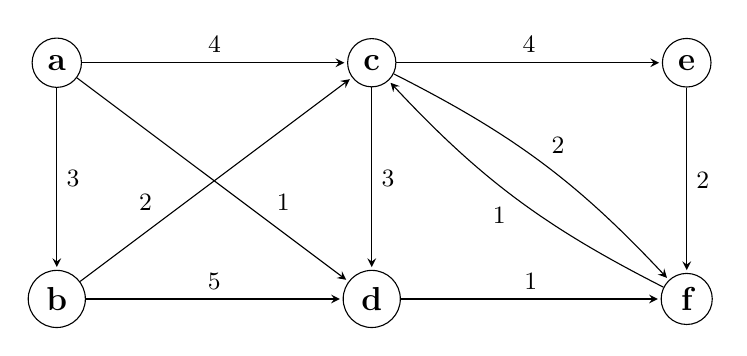
\begin{tikzpicture}[->,>=stealth,shorten >=1pt,auto,
    main node/.style={circle,draw,font=\large\bfseries}]
\node[main node] (a) at (2,1.5) {a};
\node[main node] (b) at (2,-1.5) {b};
\node[main node] (c) at (6,1.5) {c};
\node[main node] (d) at (6,-1.5) {d};
\node[main node] (e) at (10,1.5) {e};
\node[main node] (f) at (10,-1.5) {f};

\path[every node/.style={font=\small}]
(a) edge node {3} (b)
edge node {4} (c)
edge node[pos=0.7] {1} (d)
(b) edge node[pos=0.3] {2} (c)
edge node {5} (d)
(c) edge node {3} (d)
edge [bend left=10] node {2} (f)
edge node {4} (e)
(d) edge node {1} (f)
(e) edge node {2} (f)
(f) edge [bend left=10] node {1} (c);
\end{tikzpicture}
\end{center}
Hvilke kanter er med i korteste-vej træet?
\fleresvar
\mulighederstart
\svar (a,b) \korrekt
\svar (a,c)
\svar (a,d) \korrekt
\svar (b,c)
\svar (b,d)
\svar (c,d)
\svar (c,e) \korrekt
\svar (c,f)
\svar (d,f) \korrekt
\svar (e,f)
\svar (f,c) \korrekt
\mulighederslut
\forklaring{Da der kun er positive vægte kan kanterne i træet findes ved at køre Dijkstra's algoritme, der giver det angivne output (som i dette tilfælde er unikt).}


\spoergsmaal{Mindste udspændende træ}
Betragt mindste udspændende træ (eng.~\emph{minimum spanning tree}) problemet på denne graf:
\begin{center}
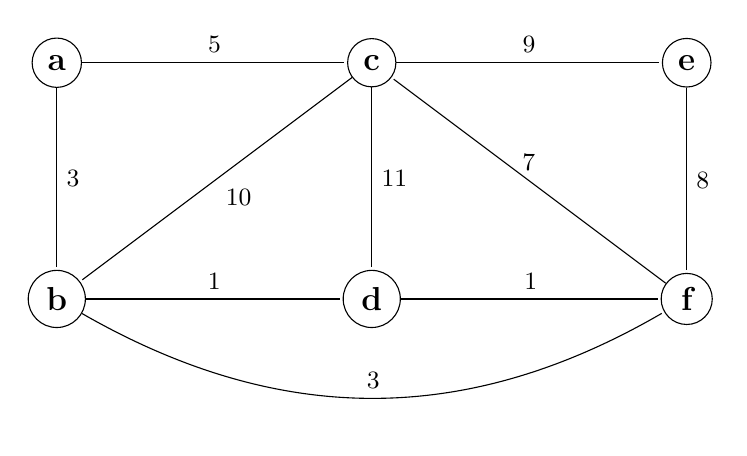
\begin{tikzpicture}[-,>=stealth,shorten >=1pt,auto,
    main node/.style={circle,draw,font=\large\bfseries}]
\node[main node] (a) at (2,1.5) {a};
\node[main node] (b) at (2,-1.5) {b};
\node[main node] (c) at (6,1.5) {c};
\node[main node] (d) at (6,-1.5) {d};
\node[main node] (e) at (10,1.5) {e};
\node[main node] (f) at (10,-1.5) {f};

\path[every node/.style={font=\small}]
(a) edge node {3} (b)
edge node {5} (c)
(b) edge node {1} (d)
edge[bend right=30] node {3} (f)
(c) edge node {11} (d)
edge node {9} (e)
edge node {10} (b)
(d) edge node {1} (f)
(e) edge node {8} (f)
(f) edge node[above] {7} (c);
\end{tikzpicture}
\end{center}
Hvilke kanter er med i mindste udspændende træ?
\fleresvar
\mulighederstart
\svar \{a,b\} \korrekt
\svar \{a,c\} \korrekt
\svar \{b,c\} 
\svar \{b,d\} \korrekt
\svar \{b,f\} 
\svar \{c,d\} 
\svar \{c,e\} 
\svar \{c,f\}
\svar \{d,f\} \korrekt
\svar \{e,f\} \korrekt
\mulighederslut
\forklaring{Mindste udspændende træ kan findes ved at køre fx Kruskal's eller Prim's algoritme og giver det angivne output (som i dette tilfælde er unikt).}



\spoergsmaal{Rød-sorte søgetræer}
Betragt dette rød-sorte binære søgetræ (eng.~\emph{red-black binary search tree}), hvor bladene er udeladt på tegningen:
%
\begin{center}
\begin{tikzpicture}[-,>=stealth,level/.style={sibling distance = 5cm/#1,
    level distance = 1cm}] 
  \node [black] {10}
      child{ node [red] {3} 
              child{ node [black] {1} 
              }
              child{ node [black] {8}
              }                            
      }
      child{ node [black] {15}
              child{ node [red] {12} 
              }
              child{ node [red] {17}
              }
          }
  ; 
  \end{tikzpicture}  
\end{center}

\medskip

Antag at vi bruger indsættelsesalgoritmen {\sc RB-Insert} fra CLRS kapitel 13 til at indsætte nøglen~9. Hvad sker med træet?
\etsvar
\mulighederstart
\svar 9 indsættes som højre barn til knude 8 og farves rød. \korrekt
\svar 9 indsættes som højre barn til knude 8 og farves sort.
\svar 9 indsættes som venstre barn til knude 12 og farves rød.
\svar 9 indsættes som venstre barn til knude 12 og farves sort.
\svar Ingen af ovenstående.
\mulighederslut
\forklaring{ {\sc RB-Insert} finder det rette sted i træet til nøglen 9, som det højre barn under knude 8. Knuden farves rød og derefter kaldes {\sc RB-Insert-Fixup}, men den terminerer uden at ændre noget fordi forældreknuden 8 er sort.
}


\spoergsmaal{Køretid for rød-sorte søgetræer}
Betragt et rød-sort binært søgetræ $T$ (eng.~\emph{red-black binary search tree}), som beskrevet i CLRS kapitel 13,
hvorpå der udføres $n_1$ {\sc Insert} operationer, $n_2$ {\sc Delete} operationer, og $n_3$ {\sc Search} operationer (sidstnævnte kaldes også ``access'' operationer).
Det totale antal operationer er $N=n_1+n_2+n_3$.
Hvilke af følgende udsagn er altid sande?
\fleresvar
\mulighederstart
\svar Den samlede tid for operationerne er $\Omega(N)$. \korrekt
\svar Den samlede tid for operationerne er $O(N \lg N)$. \korrekt
\svar Den samlede tid for operationerne er $O(n_3 + (n_1 + n_2) \lg N)$.
\svar Dybden af $T$ er højst $2\lg(n_1 + 1)$. \korrekt
\svar Alle blade i $T$ er i dybde mindst $\lfloor \lg(n_3 + 1)\rfloor$.
\svar Alle sorte knuder i $T$ har en afstand til roden, der er et lige tal.
\mulighederslut
\forklaring{ Hver operation tager mindst konstant tid, så den samlede tid er $\Omega(N)$. Antal knuder $n$ i træet er på ethvert tidspunkt højst $n_1 \leq N$. Hver operation tager altså højst $O(\lg N)$ tid, så den samlede tid er $O(N \lg N)$. I værste fald tager søgeoperationerne tid $\Omega(\lg n_1)$, dvs.~tid $\Omega(n_3\lg n_1)$ totalt, og tiden kan altså ikke begrænses af $O(n_3 + (n_1 + n_2) \lg N)$. Et rød-sort binært søgetræ kan have blade i dybde 2 uanset værdien af $n_3$, så bladene er generelt ikke i dybde mindst $\lfloor \lg(n_3 + 1)\rfloor$. Sorte knuder kan optræde på alle niveauer.
}



\spoergsmaal{Amortiseret analyse}
I denne opgave betragter vi potentialfunktionen der bruges til at analysere dynamiske tabeller i CLRS sektion 17.4.1.
Lad $\Phi_i$ betegne potentialfunktionens værdi efter $i$ {\sc Table-Insert} operationer, uden nogen {\sc Table-Delete} operationer.
Hvilke egenskaber har $\Phi_i$?
\fleresvar
\mulighederstart
\svar $\Phi_i = \Omega(1)$.\korrekt
\svar $\Phi_i = O(1)$.
\svar $\Phi_i = \Omega(i)$.
\svar $\Phi_i = O(i)$.\korrekt
\svar $\Phi_{i} \geq \Phi_{i-1}$.
\svar $\Phi_{i} \geq 0$. \korrekt
\mulighederslut
\forklaring{ $\Phi_i = 2\cdot num_i - size_i$, hvor $num_i = i$ og $size_i \geq 1$ er den aktuelle kapacitet. Vi har altid $\Phi_i \leq i$, så $\Phi_i=O(i)$, men lige efter en tabeludvidelse har vi $\Phi_i \leq 2$, dvs.~det gælder ikke at $\Phi_i = \Omega(i)$. Lige efter en tabeludvidelse har vi $\Phi_{i} < \Phi_{i-1}$. Potentialfunktionen er defineret så den er ikke-negativ, og den er positiv fra første skridt og fremefter.
}


\spoergsmaal{Del og hersk}
Hvilke af disse rekursionsligninger har løsningen
$T(n) = \Theta(n^2)$? Antag at $T(n)=1$ for $n\leq 1$.
\fleresvar
\mulighederstart
\svar $T(n) = 4 T(\lfloor n/2\rfloor ) + n \lg n$. \korrekt
\svar $T(n) = 4 T(\lfloor n/2\rfloor ) + n^2$.
\svar $T(n) = 2 T(\lfloor n/4\rfloor ) + n^2$. \korrekt
\svar $T(n) = 9 T(\lfloor n/3\rfloor ) + n^3$.
\svar $T(n) = T(n-1) + n^2$. % Kan ikke løses med master theorem i CLRS
\svar $T(n) = T(n-1) + n$. \korrekt % Kan ikke løses med master theorem i CLRS
\mulighederslut
\forklaring{ De fire første rekursionsligninger kan løses ved hjælp af master theorem, hvor nummer 1 og 3 falder i henholdsvis tilfælde 1 og 3 som giver $T(n) = \Theta(n^2)$.
De sidste ligninger kan løses med substitutionsmetoden.
I ligning 5 er der $n$ led hvor halvdelen har størrelse mindst $(n/2)^2 = n^2/4$, så $T(n)=\Omega(n^3)$.
I ligning 6 er der $n$ led af størrelse højst~$n$, hvor halvdelen har størrelse mindst $n/2$, så $T(n)=\Theta(n^2)$.
}



\multiplechoiceslut



\newpage


\section*{Skriftlige opgaver}\label{sec:written}

{\bf Skriftlige opgaver} afleveres som et Word dokument i ITX systemet.
Der er mulighed for at tegne og skrive på tablet, og indsætte i dokumentet.
\begin{itemize}
    \item Brug \emph{én side til hvert delspørgsmål, i samme rækkefølge som i opgavesættet.} 
    \item Delspørgsmålets nummer/bogstav (fx 19 eller 20.a) skal fremgå.
\end{itemize}



\section{Huffman tree (4\%)}

Vi betragter algoritmen til konstruktion af Huffman koder i CLRS sektion 16.3.

\punkt{a)}{Tegn Huffman træet som algoritmen beregner for alfabetet $C =\{a, b, c, d, e\}$ med frekvenser $f_a=5$, $f_b=8$, $f_c=3$, $f_d=7$, $f_e=1$.
Det er ikke nødvendigt at angive labels (0 og 1) på kanterne, men angiv frekvenser i blade såvel som indre knuder (se eksempel i CLRS figur~16.4).}

\forklaring{Algoritmen beregner dette træ (tegnet uden 0-1 labels på kanterne):\medskip
\begin{center}
    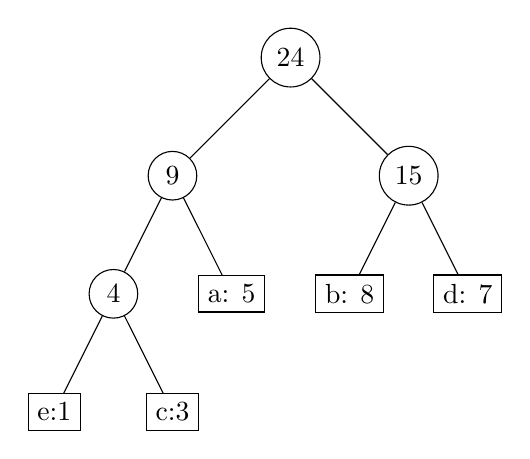
\begin{tikzpicture}[level distance=1.5cm,  level 1/.style={sibling distance=3cm},  level 2/.style={sibling distance=1.5cm}]
        \node [circle, draw] {24}
          child {node [circle, draw] {9}
            child {node [circle, draw] {4}
              child {node [rectangle, draw] {e:1}}
              child {node [rectangle, draw] {c:3}}
            }
            child {node [rectangle, draw] {a: 5}}
          }
          child {node [circle, draw] {15}
            child {node [rectangle, draw] {b: 8}}
            child {node [rectangle, draw] {d: 7}}
          };
      \end{tikzpicture}      
\end{center}
}



\section{Dynamisk programmering (10\%)}

Vi betragter følgende variant af \emph{rod cutting} problemet fra CLRS sektion 15.3.
Input er et heltal $n$ og en vektor $p$ hvor $p_i$ er fortjenesten på en stav af længde $i$.
I lighed med rod cutting skal en stav (eng.~\emph{rod}) af længde $n$ deles op i kortere stave, alle af heltalslængde, således at den totale fortjeneste maksimeres.
I modsætning til det originale rod cutting problem er der dog en omkostning på 1 for hvert snit, som skal modregnes i fortjenesten.

\medskip

{\bf Eksempel.} Antag at vi har en stav af længde $n=5$, hvor $p = (p_1,p_2,p_3,p_4,p_5) = (1,3,5,6,6)$. Hvis vi deler staven i to dele af størrelse henholdsvis 2 og 3, så bliver fortjenesten $p_2 + p_3 - 1 = 7$, hvor vi trækker $1$ fra fordi der er ét snit. Hvis vi i stedet delte i 5 dele af størrelse 1 ville fortjenesten blive $5\,p_1 - 4 = 1$.


\punkt{a)}{Skriv en rekursionsligning for fortjenesten (eng.~\emph{revenue}) $r_n$ for en stav af længde $n$.}

\forklaring{Vi har $r_0 = 0$ og med samme argument som for standard rod cutting er $r_n = \max\bigl(p_n, \max_{1\leq i \leq n-1} (p_i + r_{n-i} - 1)\bigr)$ for $n\geq 1$, hvor vi trækker 1 fra pga.~omkostningen ved snittet mellem det første stykke af længde $i$ og resten (sælges staven hel til $p_n$, laves der intet snit).}

\punkt{b)}{Lav en analyse af køretiden af algoritme, der bruger rekursionsligningen og dynamisk programmering til at beregne fortjenesten ved en stav af længde $n$. Analysen skal give en øvre grænse på køretiden som funktion af $n$ i store-$O$ notation, der er så præcis som mulig.}

\forklaring{Analysen for rod cutting kan genbruges, da rekursionsligningen har samme struktur. Ændringen påvirker kun værdierne og tiden for hvert skridt øges med højst en konstant faktor. Derfor er køretiden $O(n^2)$.}



\section{Induktionsbeviser (6\%)}

I denne opgave betragter vi $n$-kanter som disse eksempler ($n=4$ og $n=6$):
\begin{center}
\begin{tikzpicture}
  \draw (0,0) -- (2,0) -- (2,2) -- (0,2) -- (0,0);
\end{tikzpicture}
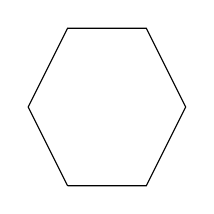
\begin{tikzpicture}
  \draw (0,0) -- (1,0) -- (1.5,1) -- (1,2) -- (0,2) -- (-0.5,1) -- (0,0);
\end{tikzpicture}
\end{center}
%
Vi er interesserede i antal \emph{diagonaler}, dvs.~linjer der forbinder to hjørner i $n$-kanterne og er helt indeholdt i figuren. En 3-kant har ingen diagonaler da alle hjørner er naboer, mens vi for $n=4$ og $n=6$ har henholdsvis 2 og 9 diagonaler.
\begin{center}
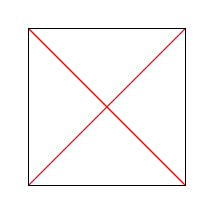
\begin{tikzpicture}
  \draw[red] (0,0) -- (2,2);
  \draw[red] (0,2) -- (2,0);
  \draw (0,0) -- (2,0) -- (2,2) -- (0,2) -- (0,0);
\end{tikzpicture}
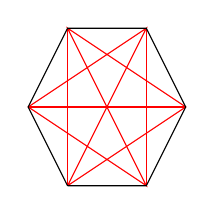
\begin{tikzpicture}
  \draw[red] (0,0) -- (0,2);
  \draw[red] (1,0) -- (1,2);
  \draw[red] (-0.5,1) -- (1.5,1);
  \draw[red] (0,0) -- (1.5,1) -- (0,2) -- (1,0) -- (-0.5,1) -- (1,2) -- (0,0) -- (1,2) -- (-0.5,1) -- (1,0) -- (0,2) -- (1.5,1);
  \draw (0,0) -- (1,0) -- (1.5,1) -- (1,2) -- (0,2) -- (-0.5,1) -- (0,0.0);
\end{tikzpicture}
\end{center}
En diagonal deler en $n$-kant en $n_1$-kant og en $n_2$ kant, der deler en kant og hvor $n_1 + n_2 = n + 2$. For eksempel deler 4-kantens diagonal den i to 3-kanter.

\punkt{a)}{Bevis ved induktion at antal diagonaler $d_n$ i en $n$-kant er lig med $n(n-3)/2$ for $n\geq 3$.
Der lægges vægt på, at argumentationen er klar og koncis.
}

\forklaring{For $n=3$ har vi $d_n = 0 = 3(3-3)/2$, hvilket etablerer basistilfældet. Antag nu at $n>3$, at udsagnet er korrekt for $n'$-kanter med $n'<n$, og betragt en $n$-kant.
Tag tre hjørner $v_1, v_2, v_3$ der ligger ved siden af hinanden, dvs.~hvor $v_1$ og $v_3$ er forbundet til $v_2$.
Fra $v_2$ kan der laves diagonaler til hver af de andre $n-3$ hjørner og
desuden kan der laves en diagonal mellem $v_1$ og $v_3$.
De resterende diagonaler ligger i den $(n-1)$-kant, der fås ved at udelade $v_2$ (og forbinde $v_1$ og $v_3$ direkte).
Ifølge induktionshypotesen har vi $d_{n-1}=(n-1)(n-4)/2$ diagonaler i denne del, dvs.
%
\[ d_n = n-3 + 1 + d_{n-1} = n-2 + (n-1)(n-4)/2 = n(n-3)/2 \enspace . \]
}



\section{Korrekthed og køretid (10\%)}\label{sec:last}

I denne opgave bruger vi matrix og vektor-notation, se evt.~CLRS appendix D.1.
Fibonaccitallene $F_0, F_1, F_2,\dots$ er defineret ved $F_0 = 0$, $F_1 = 1$, og $F_{n} = F_{n-1} + F_{n-2}$ for $n>1$.
Betragt nu matricen $A$ og søjlevektorer på formen $x = (x_1, x_2)^T$.

\[
 A =   \begin{pmatrix}
        0 & 1 \\
        1 & 1 
    \end{pmatrix}
\qquad x =   
\begin{pmatrix}
    x_1\\
    x_2 
\end{pmatrix}
\]

\punkt{a)}{Argumentér for at for $x = (F_{n-2}, F_{n-1})^T$ opfylder matrix-vektor produktet ligheden $A x = (F_{n-1}, F_{n})^T$ for $n>1$.}

\forklaring{Per definition af matrix-vektor produkter har vi:
\[
 \begin{pmatrix}
        0 & 1 \\
        1 & 1 
    \end{pmatrix}
\begin{pmatrix}
    F_{n-2}\\
    F_{n-1} 
\end{pmatrix}
=
\begin{pmatrix}
    F_{n-1}\\
    F_{n-2} + F_{n-1} 
\end{pmatrix}
=
\begin{pmatrix}
    F_{n-1}\\
    F_{n} 
\end{pmatrix},
\]
hvor den sidste lighed bruger definitionen af $F_n$.
}

\punkt{b)}{Bevis at for $x = (0,1)^T$ gælder ligheden $A^{n-1} x = (F_{n-1}, F_{n})^T$ for $n\geq 1$.}

\forklaring{
Bevis ved induktion i $n$.
Basistilfældet $n=1$ gælder da $A^{n-1} x = x = (F_0, F_1)^T$.
Antag som induktionshypotese at $A^{i-1} x = (F_{i-1}, F_{i})^T$ for $1\leq i < n$.
Da har vi%
\[
    A^{n-1} x = A(A^{n-2} x) = A (F_{n-2}, F_{n-1})^T = (F_{n-1}, F_{n})^T,
\]
hvor lighed nummer 2 bruger induktionshypotesen og lighed nummer 3 bruger del a).
}

\punkt{c)}{Argumentér for at $A^{n-1}$, og dermed også $A^{n-1} x$, kan udregnes i tid $O(\lg n)$, hvis vi antager at aritmetiske operationer tager konstant tid.}

\forklaring{
    Vi har følgende rekursionsligning:
    \begin{equation*}
        A^n = \begin{cases}
        I & \text{ hvis } n=0\\
        (A^{n/2})^2 &\text{ hvis } n > 0 \text{ er lige}\\
        A (A^{(n-1)/2})^2 &\text{ hvis } n \text{ er ulige}
        \end{cases}
    \end{equation*}
Da $A^n$ er af konstant størrelse betyder det at $A^n$ kan udregnes i konstant tid ud fra enten $A^{n/2}$ eller $A^{(n-1)/2}$.
Det giver rekursionsdybde højst $\lg(n)$, og dermed tid $O(\lg n)$.
}



\label{page:last}
